% IT6390E Knowledge Graphs -- Capstone report, Group 2
% Build: xelatex Group2_Capstone_Report.tex (twice, for references and contents)
\documentclass[11pt,a4paper]{article}

\usepackage{fontspec}
\setmainfont{STIX Two Text}
\setmonofont{Menlo}[Scale=0.82]
\usepackage[a4paper,margin=2.5cm]{geometry}
\usepackage{graphicx}
\usepackage{booktabs}
\usepackage{tabularx}
\usepackage{array}
\usepackage{caption}
\usepackage{float}
\usepackage{enumitem}
\usepackage{xcolor}
\usepackage{listings}
\usepackage{tikz}
\usetikzlibrary{arrows.meta,positioning}
\usepackage{fancyhdr}
\usepackage{microtype}
\usepackage[hidelinks]{hyperref}

\definecolor{hust}{HTML}{BF1E2E}
\definecolor{codebg}{HTML}{F5F6F8}
\captionsetup{font=small,labelfont=bf}
\setlist{itemsep=2pt,topsep=4pt}
\setlength{\parskip}{4pt}
\setlength{\emergencystretch}{2em}

\lstset{basicstyle=\ttfamily\footnotesize,backgroundcolor=\color{codebg},frame=single,rulecolor=\color{black!15},
  columns=fullflexible,keepspaces=true,breaklines=true,xleftmargin=4pt,xrightmargin=4pt,aboveskip=6pt,belowskip=6pt,
  keywordstyle=\color{hust}\bfseries}
\lstdefinelanguage{sparql}{morekeywords={SELECT,WHERE,FILTER,GROUP,BY,ORDER,DESC,LIMIT,SERVICE,COUNT,AS,PREFIX,STRSTARTS,STR},sensitive=true,morecomment=[l]{\#}}

\pagestyle{fancy}
\fancyhf{}
\fancyhead[L]{\small IT6390E Knowledge Graphs --- Group 2}
\fancyhead[R]{\small Movies Linked Open Data}
\fancyfoot[C]{\small\thepage}
\renewcommand{\headrulewidth}{0.4pt}

\newcommand{\code}[1]{\texttt{#1}}

\begin{document}

% ---------------------------------------------------------------- title page
\begin{titlepage}
\centering

\includegraphics[width=0.42\textwidth]{fig/logo-soict-hust.png}\par\vspace{1.2cm}
{\large HANOI UNIVERSITY OF SCIENCE AND TECHNOLOGY\par}
{\large SCHOOL OF INFORMATION AND COMMUNICATION TECHNOLOGY\par}
\vspace{2.2cm}
{\large\bfseries IT6390E --- KNOWLEDGE GRAPHS\par}
{\large Capstone Project Report\par}
\vspace{1.2cm}
{\color{hust}\rule{0.6\textwidth}{1pt}\par}\vspace{0.5cm}
{\LARGE\bfseries Movies Linked Open Data:\par}
\vspace{0.2cm}
{\Large A Five-Star Knowledge Graph of 250 Films\\ Linked to Wikidata and DBpedia\par}
\vspace{0.5cm}{\color{hust}\rule{0.6\textwidth}{1pt}\par}
\vspace{2cm}
{\large Group 2\par}\vspace{0.4cm}
\begin{tabular}{l}
Đỗ Tuấn Minh\\
Nguyễn Tiến Đức\\
Hoàng Huy Chiến
\end{tabular}
\vfill
{\small Source code and data: \url{https://github.com/minhdo2207/it6390e-lod-capstone}\par}
\vspace{0.4cm}
{\large Hanoi, October 2026\par}
\end{titlepage}

% ---------------------------------------------------------------- abstract
\begin{abstract}
\noindent
This report presents a Linked Open Data application in the movie domain that reaches all five stars of the deployment scheme proposed by Berners-Lee. We designed a small OWL ontology that reuses schema.org, FOAF, the DBpedia ontology and Dublin Core, collected the 250 best-rated films of the TMDB 5000 dataset, converted them to RDF with stable URIs, and linked films and people to Wikidata and DBpedia. Linking matches on the TMDB identifiers that Wikidata already stores instead of on titles, which produced 920 \code{owl:sameAs} links to Wikidata and 912 to DBpedia. A manual evaluation on a random sample of 30 resources measured a precision of 100\% for Wikidata and 96.7\% for DBpedia; the single error revealed that DBpedia redirect resources carry stale \code{owl:sameAs} statements, which we then excluded. Defined classes and one SWRL rule allow the HermiT reasoner to infer 29 action films, 16 comedies, 32 award-winning directors and 5 actor-directors, and a deliberately contradictory record is detected as an inconsistency. The resulting graph of 12,013 triples is queried with 21 SPARQL queries, ten of which are federated queries that retrieve facts from Wikidata and DBpedia at query time.

\medskip\noindent\textbf{Keywords:} Linked Open Data, ontology engineering, OWL, SWRL, entity linking, SPARQL federation.
\end{abstract}

\tableofcontents
\newpage

% ---------------------------------------------------------------- 1
\section{Introduction}

Linked Open Data (LOD) publishes structured data on the Web so that it can be combined with other datasets: entities are named by HTTP URIs, described in RDF, and connected to entities in other datasets~\cite{bizer2009linked}. Berners-Lee's five-star scheme grades how far a dataset goes on this path~\cite{fivestar}: openly licensed data on the Web (one star), machine-readable structure (two), a non-proprietary format (three), W3C standards with URIs for things (four), and links to other datasets (five).

The capstone asks for a LOD application in a chosen domain, built in five steps: (1) define an ontology, (2) collect data, (3) convert the data to four-star data, (4) link it to other datasets to reach five stars, and (5) provide a SPARQL query interface. We chose the movie domain for two reasons. Open movie data is plentiful, and the two central hubs of the LOD cloud, DBpedia~\cite{dbpedia} and Wikidata~\cite{wikidata}, describe films, directors and actors in depth, which makes the fifth star reachable within the project time.

The contributions of this work are:
\begin{itemize}
  \item an ontology with nine core classes, defined classes and a SWRL rule, plus an n-ary model of cast roles (Section~\ref{sec:ontology});
  \item a reproducible pipeline from the TMDB 5000 dataset to linked RDF (Sections~\ref{sec:data}--\ref{sec:rdf});
  \item an identifier-based linking method with a manual precision evaluation and an analysis of a failure mode of DBpedia links (Section~\ref{sec:linking});
  \item a query interface with local, n-ary and federated SPARQL queries, and a reasoning evaluation in Protégé (Sections~\ref{sec:sparql}--\ref{sec:reasoning}).
\end{itemize}

\noindent Table~\ref{tab:stars} summarises how the project meets each level of the scheme.

\begin{table}[H]
\centering\small
\caption{The five-star scheme applied to this project.}\label{tab:stars}
\begin{tabularx}{\textwidth}{@{}lXX@{}}
\toprule
Stars & Requirement & This project \\
\midrule
$\star$ & On the Web under an open licence & Public repository; RDF under CC BY-NC 4.0, code under MIT \\
$\star\star$ & Machine-readable structured data & Cleaned dataset as a CSV table \\
$\star\star\star$ & Non-proprietary format & CSV and Turtle \\
$\star\star\star\star$ & URIs and W3C standards & A URI for every film, person, genre, studio, country and cast role; RDF, OWL, SPARQL \\
$\star\star\star\star\star$ & Links to other data & 920 \code{owl:sameAs} links to Wikidata, 912 to DBpedia \\
\bottomrule
\end{tabularx}
\end{table}

% ---------------------------------------------------------------- 2
\section{Ontology Design}\label{sec:ontology}

\subsection{Method and competency questions}

We followed a lightweight version of Methontology~\cite{methontology}: specification through competency questions, conceptualisation as a glossary of terms, reuse of existing vocabularies, then implementation in OWL~2 with Protégé. Competency questions, as proposed by Grüninger and Fox~\cite{gruninger1995}, were fixed before any modelling. They determined which classes and properties were needed, and each was later implemented as a SPARQL query (Section~\ref{sec:sparql}):
\begin{enumerate}
  \item Who directed movie $X$? \hfill (query 1)
  \item Which movies were released after year $Y$? \hfill (query 2)
  \item Which director has the most movies? \hfill (query 3)
  \item Which movies feature actor $Y$? \hfill (query 5)
  \item Which character did an actor play, and how high was the actor billed? \hfill (queries 16--17)
\end{enumerate}

\subsection{Classes and properties}

Following LOD best practice, existing vocabulary terms were reused before new ones were minted~\cite{bizer2009linked}: \code{schema:Movie}, \code{foaf:Person}, \code{dbo:director}, \code{dbo:starring}, \code{dc:title} and \code{foaf:name}. Local terms in the namespace \code{http://it6390e-group2.example.org/ontology/} (prefix \code{ont:}) cover what these vocabularies lack. Figure~\ref{fig:ontology} shows the core structure and Table~\ref{tab:terms} lists the terms.

\begin{figure}[H]
\centering
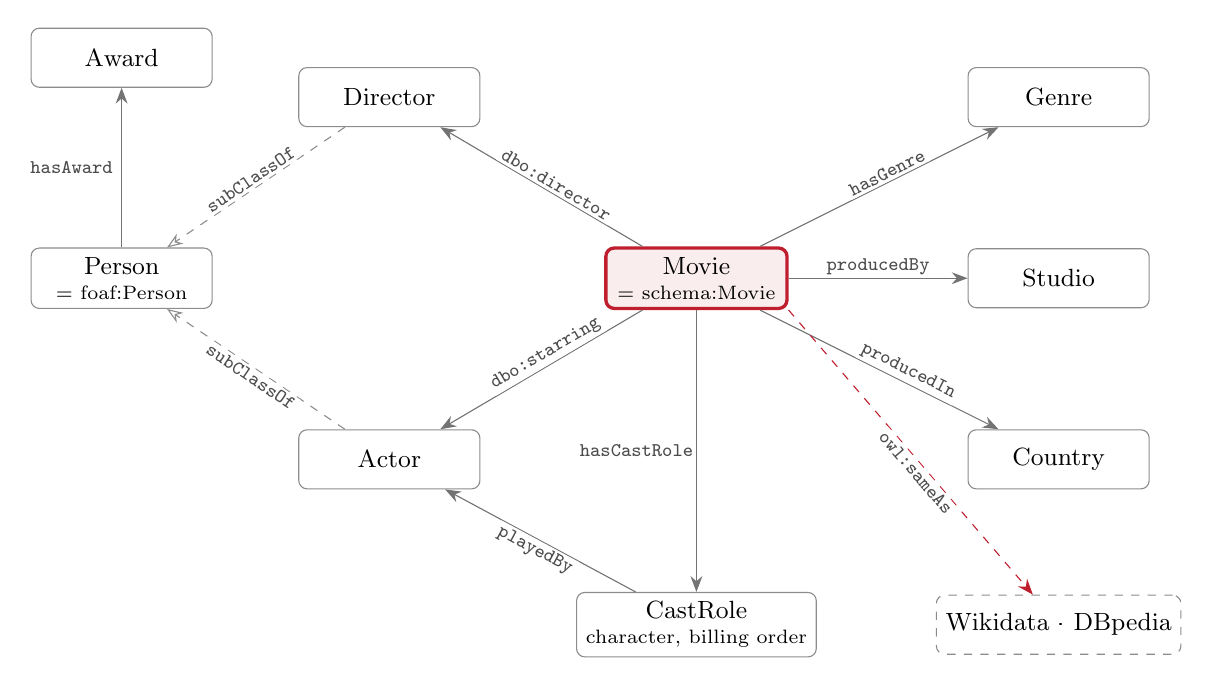
\begin{tikzpicture}[
  cls/.style={draw=black!45,rounded corners=3pt,minimum width=2.3cm,minimum height=0.75cm,font=\small,align=center},
  main/.style={cls,draw=hust,very thick,fill=hust!8},
  ext/.style={cls,dashed},
  rel/.style={-{Stealth[length=2mm]},black!55},
  sub/.style={-{Stealth[length=2mm,open]},black!45,dashed},
  lab/.style={font=\scriptsize\ttfamily,text=black!70,fill=white,inner sep=1pt}]
\node[main] (movie) at (0,0) {Movie\\[-2pt]{\scriptsize = schema:Movie}};
\node[cls] (director) at (-3.9,2.3) {Director};
\node[cls] (actor) at (-3.9,-2.3) {Actor};
\node[cls] (person) at (-7.3,0) {Person\\[-2pt]{\scriptsize = foaf:Person}};
\node[cls] (award) at (-7.3,2.8) {Award};
\node[cls] (genre) at (4.6,2.3) {Genre};
\node[cls] (studio) at (4.6,0) {Studio};
\node[cls] (country) at (4.6,-2.3) {Country};
\node[cls] (role) at (0,-4.4) {CastRole\\[-2pt]{\scriptsize character, billing order}};
\node[ext] (links) at (4.6,-4.4) {Wikidata · DBpedia};
\draw[rel] (movie) -- node[lab,above,sloped,pos=0.45] {dbo:director} (director);
\draw[rel] (movie) -- node[lab,above,sloped,pos=0.45] {dbo:starring} (actor);
\draw[sub] (director) -- node[lab,above,sloped] {subClassOf} (person);
\draw[sub] (actor) -- node[lab,below,sloped] {subClassOf} (person);
\draw[rel] (person) -- node[lab,left,xshift=-2pt] {hasAward} (award);
\draw[rel] (movie) -- node[lab,above,sloped,pos=0.55] {hasGenre} (genre);
\draw[rel] (movie) -- node[lab,above] {producedBy} (studio);
\draw[rel] (movie) -- node[lab,above,sloped,pos=0.6] {producedIn} (country);
\draw[rel] (movie) -- node[lab,left,pos=0.5] {hasCastRole} (role);
\draw[rel] (role) -- node[lab,below,sloped] {playedBy} (actor);
\draw[rel,dashed,hust] (movie.south east) -- node[lab,below,sloped,pos=0.55] {owl:sameAs} (links);
\end{tikzpicture}
\caption{Core classes and properties of the ontology. Dashed open arrows denote \code{rdfs:subClassOf}; the dashed red arrow denotes the \code{owl:sameAs} links to external datasets.}\label{fig:ontology}
\end{figure}

\begin{table}[H]
\centering\small
\caption{Main terms of the ontology (\code{ontology/movies.ttl}).}\label{tab:terms}
\begin{tabularx}{\textwidth}{@{}>{\raggedright\arraybackslash}p{4.4cm}l>{\raggedright\arraybackslash}X@{}}
\toprule
Term & Kind & Definition / source \\
\midrule
\code{Movie} & class & equivalent to \code{schema:Movie} \\
\code{Person} & class & equivalent to \code{foaf:Person} \\
\code{Director}, \code{Actor} & class & subclasses of \code{Person} \\
\code{Genre}, \code{Studio}, \code{Country}, \code{Award} & class & local classes \\
\code{CastRole} & class & one actor appearing in one movie (n-ary relation) \\
\code{dbo:director}, \code{dbo:starring} & object property & Movie $\rightarrow$ Director / Actor (DBpedia ontology) \\
\code{hasGenre}, \code{producedBy}, \code{producedIn} & object property & Movie $\rightarrow$ Genre / Studio / Country \\
\code{hasAward} & object property & Person $\rightarrow$ Award \\
\code{hasCastRole}, \code{roleInMovie}, \code{playedBy} & object property & Movie $\leftrightarrow$ CastRole (inverses), CastRole $\rightarrow$ Actor (functional) \\
\code{releaseYear} & datatype property & Movie $\rightarrow$ \code{xsd:integer} \\
\code{characterName}, \code{billingOrder} & datatype property & character played, position in the credits \\
\bottomrule
\end{tabularx}
\end{table}

\noindent \code{releaseYear} uses \code{xsd:integer} rather than \code{xsd:gYear} because HermiT does not support \code{xsd:gYear} in its datatype map.

\subsection{Defined classes and a SWRL rule}

Three classes are defined by necessary and sufficient conditions, so that their members are inferred rather than asserted. In Manchester syntax:
\par\noindent\begin{minipage}{\linewidth}\begin{lstlisting}
ActionMovie          EquivalentTo  hasGenre value genre_action
ComedyMovie          EquivalentTo  hasGenre value genre_comedy
ComedyMovie          DisjointWith  ActionMovie
AwardWinningDirector EquivalentTo  Director and (hasAward some Award)
\end{lstlisting}\end{minipage}\par
The first two follow the pattern of \code{VegetarianPizza} in the Protégé pizza tutorial. The class \code{ActorDirector}, a person who directed and starred in the same movie, cannot be expressed as an OWL~2 class expression: it requires the same individual to fill two different properties of one movie, and OWL property chains can only derive a property, not test a join of this kind. It is therefore derived by a SWRL rule~\cite{swrl}:
\par\noindent\begin{minipage}{\linewidth}\begin{lstlisting}
Movie(?m) ^ dbo:director(?m, ?p) ^ dbo:starring(?m, ?p) -> ActorDirector(?p)
\end{lstlisting}\end{minipage}\par

\subsection{Cast roles as an n-ary relation}

The binary property \code{dbo:starring} links a movie to an actor but cannot record the character played or the billing position. Following the W3C note on n-ary relations~\cite{naryrel}, each appearance of an actor in a movie is reified as a \code{CastRole} individual carrying \code{characterName} and \code{billingOrder}. \code{dbo:starring} is retained for compatibility, and the property chain axiom $\code{hasCastRole} \circ \code{playedBy} \sqsubseteq \code{dbo:starring}$ lets a reasoner derive it from the roles, so that the two representations cannot diverge. A consistency query confirms that both describe the same 750 actor--movie pairs.

\subsection{A modelling trade-off}

Under OntoClean~\cite{ontoclean}, \code{Director} and \code{Actor} are anti-rigid roles rather than rigid types: being a director is not essential to a person. Modelling them as subclasses of \code{Person} therefore violates the rigidity constraint, and a cleaner design would attach roles to persons through a property such as \code{hasRole}. We kept the subclass design to limit the scope of the capstone; for actors, the \code{CastRole} node already provides a role-based model.

% ---------------------------------------------------------------- 3
\section{Data Collection}\label{sec:data}

The data source is the Kaggle ``TMDB 5000 Movie Dataset''~\cite{tmdb5000}, two CSV files generated from the TMDb API that describe 4,803 films and their cast and crew. The script \code{prepare\_movies\_csv.py} keeps films with at least 1,000 votes, sorts them by average rating and selects the first 250, discarding rows without a title, release date or director. For each film it keeps the TMDB identifier, title, release year, runtime, director, the primary genre, and the three first-billed actors with their characters, together with the first production company and country.

The resulting dataset covers films released between 1939 and 2016 and contains 250 films, 672 distinct people (156 directors and 522 actors), 17 genres, 99 studios and 16 countries, with no empty cells. Figure~\ref{fig:genres} shows the distribution of primary genres. Only the primary genre is converted to RDF; Section~\ref{sec:reasoning} explains why.

\begin{figure}[H]
\centering
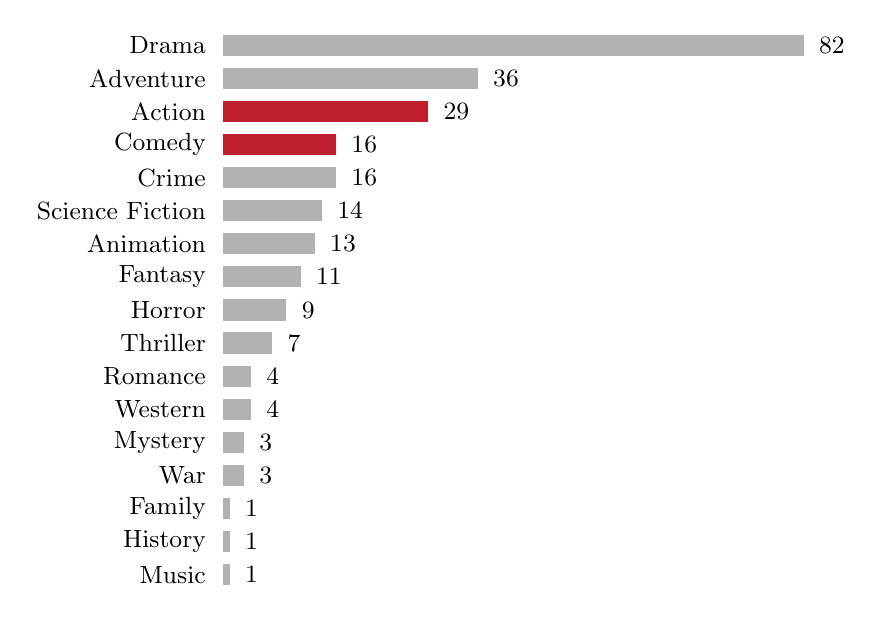
\begin{tikzpicture}[x=0.09cm,y=0.42cm,font=\small]
\foreach \g/\n/\i in {Drama/82/1,Adventure/36/2,Action/29/3,Comedy/16/4,Crime/16/5,Science Fiction/14/6,Animation/13/7,Fantasy/11/8,Horror/9/9,Thriller/7/10,Romance/4/11,Western/4/12,Mystery/3/13,War/3/14,Family/1/15,History/1/16,Music/1/17}{
  \pgfmathsetmacro{\yy}{-\i}
  \node[anchor=east] at (-1,\yy) {\g};
  \ifnum\i=3 \fill[hust] (0,\yy-0.32) rectangle (\n,\yy+0.32);
  \else\ifnum\i=4 \fill[hust] (0,\yy-0.32) rectangle (\n,\yy+0.32);
  \else \fill[black!30] (0,\yy-0.32) rectangle (\n,\yy+0.32); \fi\fi
  \node[anchor=west] at (\n+0.8,\yy) {\n};
}
\end{tikzpicture}
\caption{Films per primary genre (250 films). Red: the two genres behind the defined classes \code{ActionMovie} and \code{ComedyMovie}.}\label{fig:genres}
\end{figure}

\noindent The data comes from the TMDb API and is not endorsed by TMDb. TMDb's terms restrict commercial use, so the derived RDF is published under CC BY-NC 4.0 with attribution.

% ---------------------------------------------------------------- 4
\section{Conversion to Four-Star RDF}\label{sec:rdf}

\subsection{Pipeline}

Four Python scripts, based on RDFLib, turn the source files into linked Turtle; every step can be rerun from scratch:
\begin{enumerate}
  \item \code{prepare\_movies\_csv.py} selects the films and writes \code{movies.csv};
  \item \code{csv\_to\_rdf.py} converts each row to RDF and writes \code{movies.ttl};
  \item \code{link\_wikidata\_dbpedia.py} adds the \code{owl:sameAs} links and a link report (Section~\ref{sec:linking});
  \item \code{add\_awards.py} adds Academy Award for Best Director wins from Wikidata (32 people).
\end{enumerate}

\subsection{URI design and mapping}

Resources are named under \code{http://it6390e-group2.example.org/}: \code{resource/movie/\{tmdb id\}}, \code{resource/person/\{tmdb id\}} and \code{resource/role/\{movie id\}-\{actor id\}}; genres, studios and countries are named after slugs of their labels. Reusing TMDB identifiers keeps the URIs stable across runs and, as Section~\ref{sec:linking} shows, provides the key for linking. Genre individuals are named \code{genre\_action}, \code{genre\_comedy}, etc., so that they coincide with the individuals used in the \code{hasValue} restrictions. Table~\ref{tab:mapping} gives the mapping and Listing~\ref{lst:turtle} one resulting resource.

\begin{table}[H]
\centering\small
\caption{Mapping from CSV columns to RDF.}\label{tab:mapping}
\begin{tabularx}{\textwidth}{@{}>{\raggedright\arraybackslash}p{4.2cm}>{\raggedright\arraybackslash}Xl@{}}
\toprule
CSV column & RDF & Vocabulary \\
\midrule
\code{id} & \code{ex:movie/\{id\} a schema:Movie} & schema.org \\
\code{title} & \code{dc:title} & Dublin Core \\
\code{year} & \code{ont:releaseYear} (\code{xsd:integer}) & local \\
\code{director\_id}, \code{director\_name} & \code{dbo:director ex:person/\{id\}}; \code{foaf:name} & DBpedia, FOAF \\
\code{cast\_ids}, \code{cast\_names}, \code{cast\_characters} & \code{dbo:starring}; \code{ont:CastRole} with \code{characterName}, \code{billingOrder} & DBpedia, local \\
\code{genre} & \code{ont:hasGenre ont:genre\_\{name\}} & local \\
\code{studio}, \code{country} & \code{ont:producedBy}, \code{ont:producedIn} & local \\
\bottomrule
\end{tabularx}
\end{table}

\par\noindent\begin{minipage}{\linewidth}\begin{lstlisting}[caption={The film \emph{The Prestige} in \code{movies\_linked.ttl} (URIs shortened).},label={lst:turtle},captionpos=b]
ex:movie/1124 a schema:Movie ;
    dc:title "The Prestige" ;  ont:releaseYear 2006 ;
    dbo:director ex:person/525 ;
    dbo:starring ex:person/3894, ex:person/3895, ex:person/6968 ;
    ont:hasCastRole ex:role/1124-3894, ex:role/1124-3895, ex:role/1124-6968 ;
    ont:hasGenre ont:genre_drama ;
    ont:producedBy ont:studio/warner-bros ;
    ont:producedIn ont:country/united-states-of-america ;
    owl:sameAs dbr:The_Prestige_(film), wd:Q46551 .
\end{lstlisting}\end{minipage}\par

\noindent The linked data contains 11,868 triples; together with the ontology and the awards, the graph has 12,013 triples describing 250 films, 672 people and 750 cast roles. Data in RDF, serialised in Turtle, with a URI for every entity, satisfies the fourth star.

% ---------------------------------------------------------------- 5
\section{Linking to Wikidata and DBpedia}\label{sec:linking}

\subsection{A failed baseline: matching on title and year}

The obvious approach is to look up each film on DBpedia by its label and release year. On a sample of eight films this matched none. Inspection showed that DBpedia film resources carry no \code{dbo:releaseDate}, so the year filter never succeeds; titles are in any case ambiguous because of remakes and sequels.

\subsection{Identifier-based matching}

Wikidata records the TMDB identifier of films (property P4947) and of people (P4985). Since our URIs end in that identifier, linking becomes an exact lookup:
\begin{enumerate}
  \item For batches of 100 identifiers, one SPARQL query to the Wikidata Query Service retrieves the items carrying them. A link is added only if exactly one item carries the identifier.
  \item The DBpedia resource is taken from DBpedia's own \code{owl:sameAs} statements pointing at the Wikidata item, restricted to resources typed \code{dbo:Film} or \code{dbo:Person}. This restriction is needed because these statements are noisy: the item for one film also had a soundtrack album and unrelated pages attached. Among the candidates, the resource named after the item's English Wikipedia article is chosen.
  \item Ambiguous cases are left unlinked rather than guessed. Two occurred: \emph{Apocalypse Now} shares its TMDB identifier with the \emph{Redux} cut, and the actor J.\,K. Simmons has a duplicate Wikidata item.
\end{enumerate}
The result is 920 links to Wikidata (249 of 250 films, 671 of 672 people) and 912 to DBpedia (249 films, 663 people).

\subsection{Evaluation}

To estimate precision we drew a reproducible random sample of 15 films and 15 people (fixed seed 42) and checked every linked Wikidata and DBpedia page by hand, comparing release year and director for films, and occupation and date of birth for people. Table~\ref{tab:precision} reports the results.

\begin{table}[H]
\centering\small
\caption{Precision of the links on a random sample of 30 resources.}\label{tab:precision}
\begin{tabular}{@{}lcc@{}}
\toprule
Target & Correct links & Precision \\
\midrule
Wikidata & 30 / 30 & 100\% \\
DBpedia & 29 / 30 & 96.7\% \\
\bottomrule
\end{tabular}
\end{table}

\subsection{Failure analysis: redirect resources}

The only wrong link, \code{dbr:Alakina\_Mann}, was a redirect resource: the Wikipedia article about the actress had been merged into the article about the film \emph{The Others}, while DBpedia kept the old resource's type and \code{owl:sameAs} statement. A scan of all 916 DBpedia links at that time found seven redirect resources, four of which led to a different entity (Alakina Mann $\rightarrow$ the film \emph{The Others}; Joel Coen $\rightarrow$ Coen brothers; Anthony Russo $\rightarrow$ Russo brothers; Lilly Wachowski $\rightarrow$ The Wachowskis). Such links assert identity between distinct entities, the misuse of \code{owl:sameAs} documented by Halpin et al.~\cite{halpin2010sameas}. The linking script now skips redirect resources and follows a redirect only when its target is the resource named after the item's English article, that is, when the redirect is a plain rename. After this correction none of the 912 DBpedia links is a redirect.

% ---------------------------------------------------------------- 6
\section{SPARQL Query Interface}\label{sec:sparql}

The graph is queried through two interfaces: \code{sparql\_cli.py}, a terminal tool over RDFLib that runs stored or ad-hoc queries, and the Snap SPARQL Query plugin inside Protégé (the SPARQL plugin bundled with Protégé 5.6.9 fails to load because of a missing library). Snap SPARQL evaluates queries through the active reasoner, so it also returns inferred facts: asking for the instances of \code{ont:ActionMovie} returns the same 87 IRIs as the DL query in Section~\ref{sec:reasoning}. Twenty-one queries are provided (Table~\ref{tab:queries}).

\begin{table}[H]
\centering\small
\caption{Query sets.}\label{tab:queries}
\begin{tabularx}{\textwidth}{@{}llX@{}}
\toprule
Queries & File & Purpose \\
\midrule
1--5 (local) & \code{sample\_queries.rq} & competency questions; films linked to DBpedia \\
16--21 (cast roles) & \code{castrole\_queries.rq} & characters and billing order; agreement between roles and \code{dbo:starring} \\
6--15 (federated) & \code{federated\_queries.rq} & facts retrieved from Wikidata and DBpedia with \code{SERVICE} \\
\bottomrule
\end{tabularx}
\end{table}

\paragraph{Competency question 3.} The query below ranks directors by number of films. Steven Spielberg leads with 8 films, followed by Quentin Tarantino and Christopher Nolan with 7, and Martin Scorsese and David Fincher with 6.
\par\noindent\begin{minipage}{\linewidth}\begin{lstlisting}[language=sparql]
SELECT ?directorName (COUNT(?movie) AS ?movieCount) WHERE {
  ?movie dbo:director ?d .
  ?d foaf:name ?directorName .
}
GROUP BY ?directorName ORDER BY DESC(?movieCount) LIMIT 5
\end{lstlisting}\end{minipage}\par

\paragraph{Cast roles.} Query 16 lists the cast of a film through \code{CastRole}. For \emph{The Dark Knight} it returns Christian Bale as Bruce Wayne (billed first), Heath Ledger as the Joker and Aaron Eckhart as Harvey Dent, information that the binary \code{dbo:starring} link cannot hold.

\paragraph{Federated queries.} Our data stores no dates of birth. Query 6 follows a director's \code{owl:sameAs} link and retrieves the date and place of birth from Wikidata with a \code{SERVICE} clause, then joins them with the director's films in our graph. For Christopher Nolan it returns 30 July 1970, London, with seven films from \emph{Memento} (2000) to \emph{Interstellar} (2014). A simplified form:
\par\noindent\begin{minipage}{\linewidth}\begin{lstlisting}[language=sparql]
SELECT ?title ?year ?birthDate WHERE {
  ?d foaf:name "Christopher Nolan" ; owl:sameAs ?wd .
  FILTER(STRSTARTS(STR(?wd), "http://www.wikidata.org/entity/"))
  ?movie dbo:director ?d ; dc:title ?title ; ont:releaseYear ?year .
  SERVICE <https://query.wikidata.org/sparql> { ?wd wdt:P569 ?birthDate . }
}
\end{lstlisting}\end{minipage}\par
Query 7 applies the same idea to every director with at least six films and computes the age at their earliest film in our data (for example, 29 for Steven Spielberg, born 1946, with \emph{Jaws} in 1975). These queries are only possible because of the fifth-star links.

% ---------------------------------------------------------------- 7
\section{Reasoning Evaluation}\label{sec:reasoning}

No film or person in the data is asserted to belong to a defined class. We evaluated the reasoning in two ways: with HermiT~\cite{hermit} run from a script (\code{check\_reasoning.py}, through owlready2) and interactively in Protégé~5.6.9~\cite{protege}. For Protégé, \code{make\_protege\_demo.py} merges the ontology, the linked data and the awards into a single file, since Protégé reasons over one ontology at a time. Classification takes HermiT about three minutes on this file, most of it spent on computing the instances of all object properties.

\begin{table}[H]
\centering\small
\caption{Inferred class members. Protégé lists every IRI of an individual, so linked individuals appear up to three times.}\label{tab:reasoning}
\begin{tabular}{@{}lcc@{}}
\toprule
Class & Our resources & Names listed in Protégé \\
\midrule
\code{ActionMovie} & 29 films & 87 \\
\code{ComedyMovie} & 16 films & 48 \\
\code{AwardWinningDirector} & 32 directors & 95 \\
\code{ActorDirector} (with the SWRL rule) & 5 people & 15 \\
\code{CastRole} & 750 roles & 750 \\
\bottomrule
\end{tabular}
\end{table}

Both runs give the same counts (Table~\ref{tab:reasoning}). The larger numbers in Protégé are a direct effect of linking: \code{owl:sameAs} makes each film or person the same individual as its Wikidata and DBpedia IRIs, and Protégé lists all of them (one director has no DBpedia link, hence 95 rather than 96). The SWRL rule classifies Clint Eastwood, Kevin Costner, Mel Gibson, Terry Gilliam and Woody Allen as actor-directors. Figures~\ref{fig:actionmovie} and~\ref{fig:actordirector} show two of these results.

\begin{figure}[H]
\centering
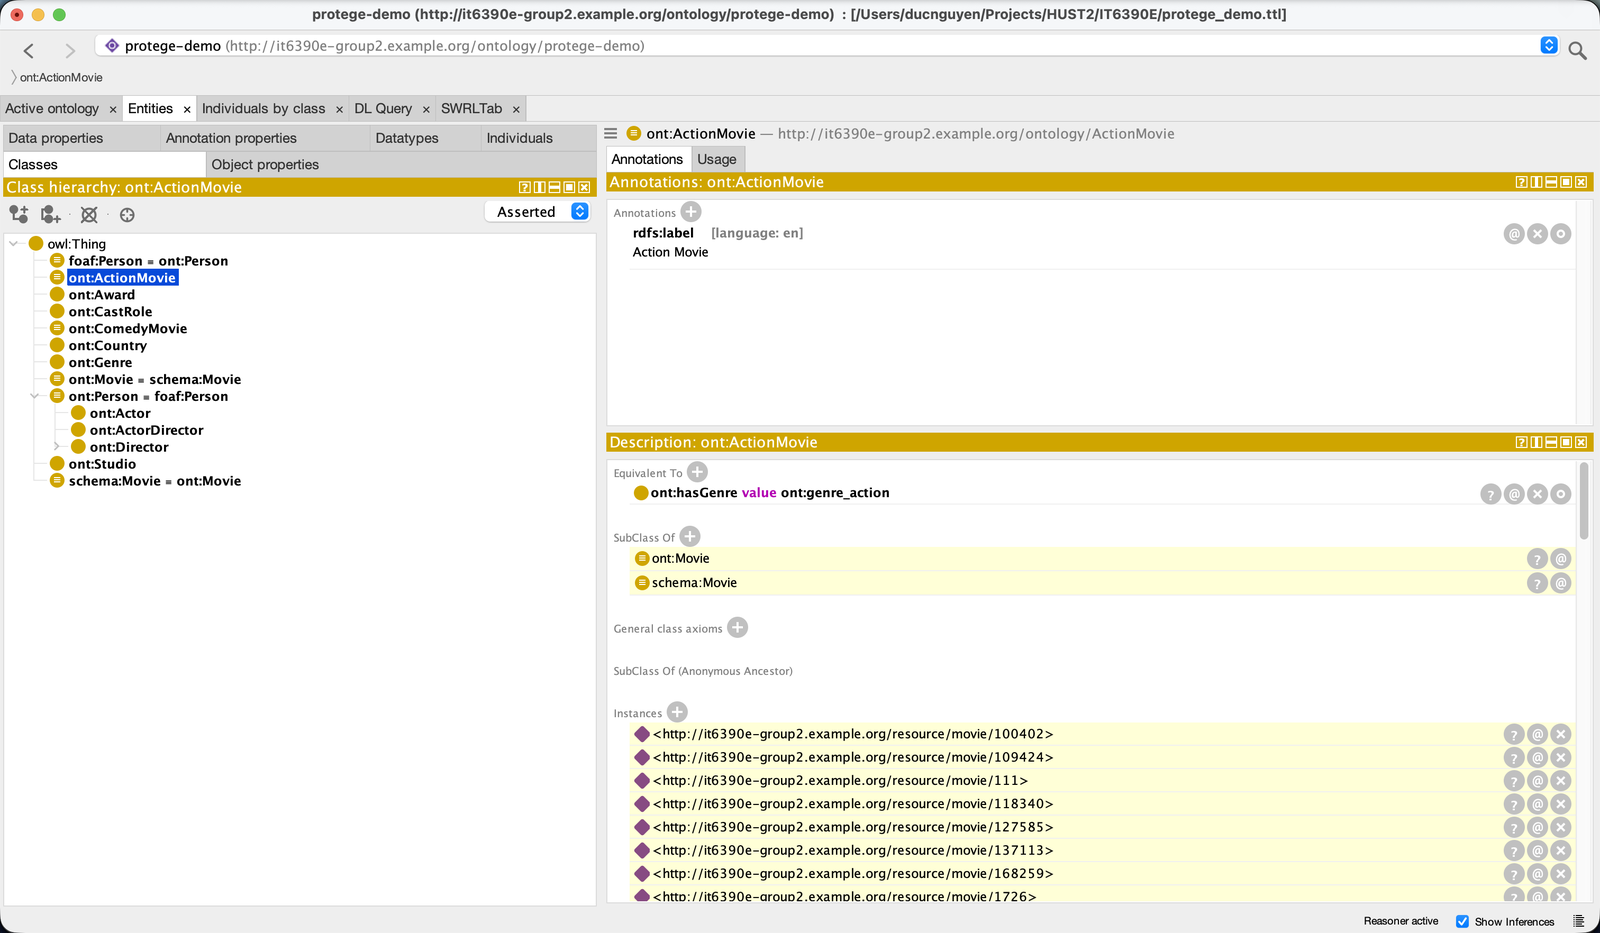
\includegraphics[width=0.92\textwidth]{fig/fig1-actionmovie.png}
\caption{\code{ont:ActionMovie} in Protégé: its definition \code{hasGenre value genre\_action} and its instances inferred by HermiT (highlighted rows).}\label{fig:actionmovie}
\end{figure}

\begin{figure}[H]
\centering
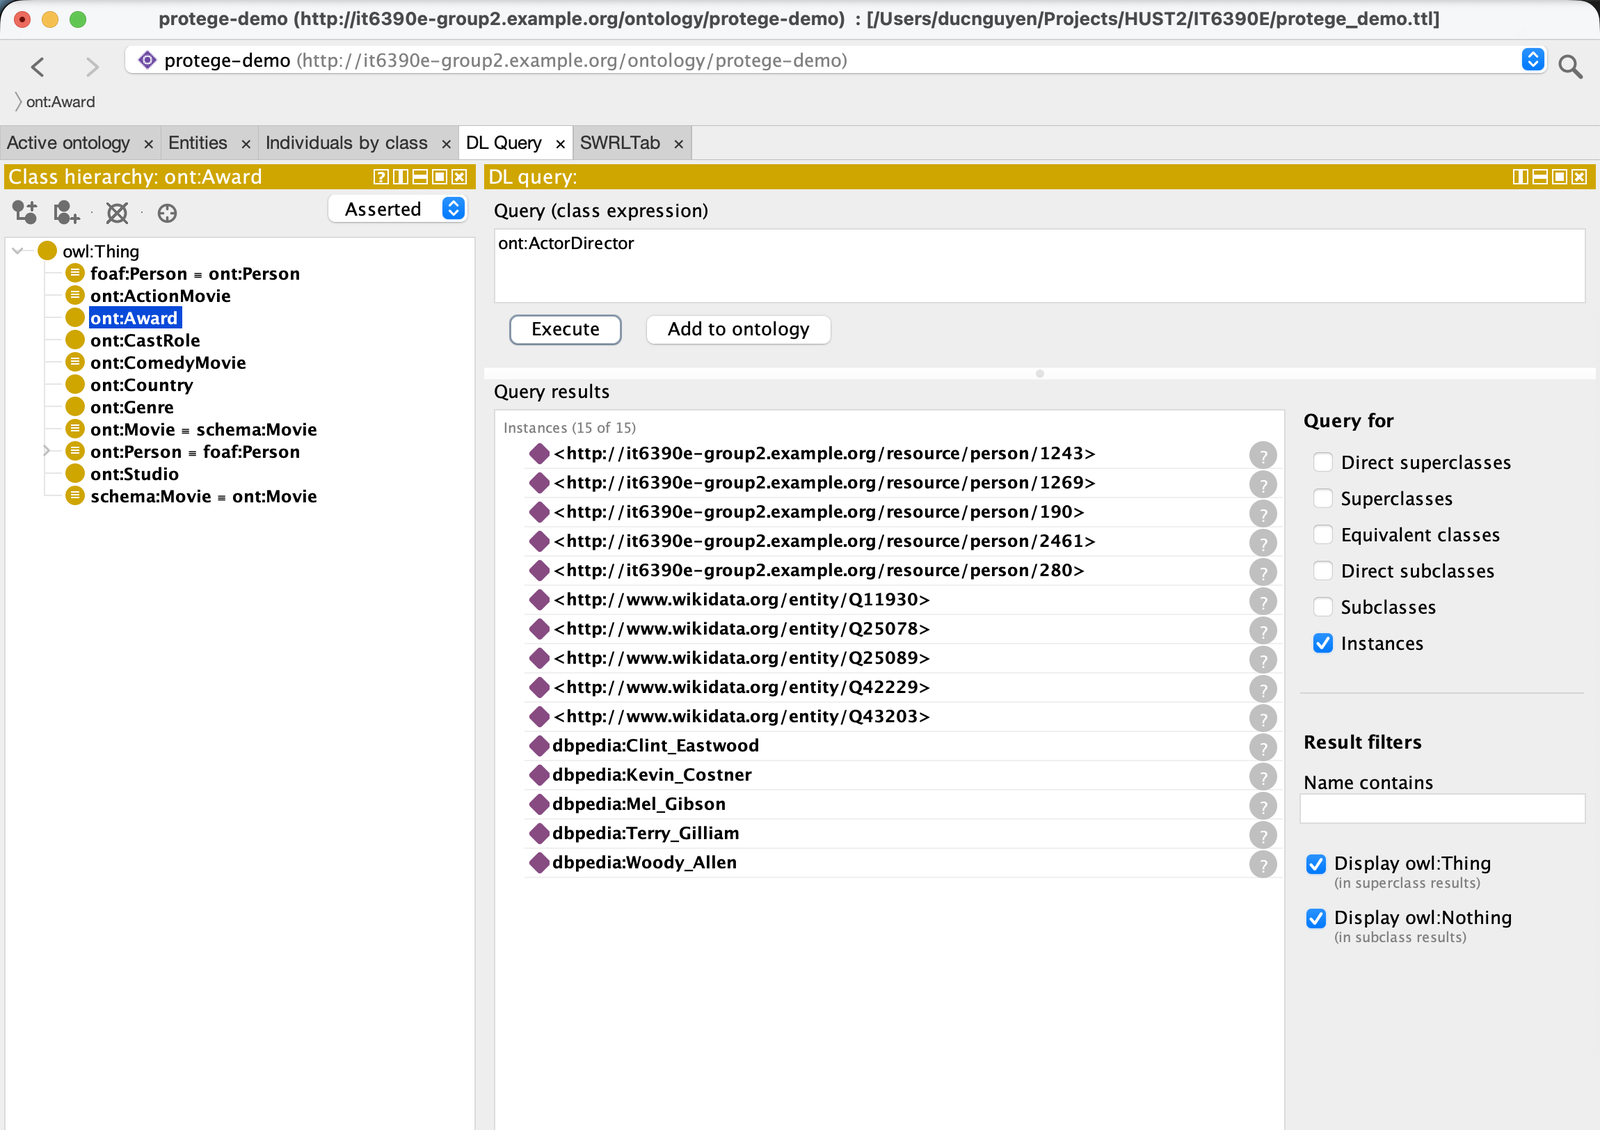
\includegraphics[width=0.82\textwidth]{fig/fig2-actordirector.png}
\caption{DL query \code{ont:ActorDirector} after adding the SWRL rule: five people, each listed under three IRIs.}\label{fig:actordirector}
\end{figure}

\paragraph{Inconsistency detection.} To test the disjointness axiom, a second file adds one film asserted to have both the Action and the Comedy genre. HermiT reports the ontology as inconsistent within seconds, and Protégé's explanation (Figure~\ref{fig:explain}) identifies the five axioms responsible: the disjointness of \code{ActionMovie} and \code{ComedyMovie}, the two \code{hasValue} definitions, and the two genre assertions. Under the open world assumption, nothing would make the two genres incompatible without the explicit disjointness axiom. The same axiom explains why only the primary genre is converted: with all genres, every action comedy would make the ontology inconsistent.

\begin{figure}[H]
\centering
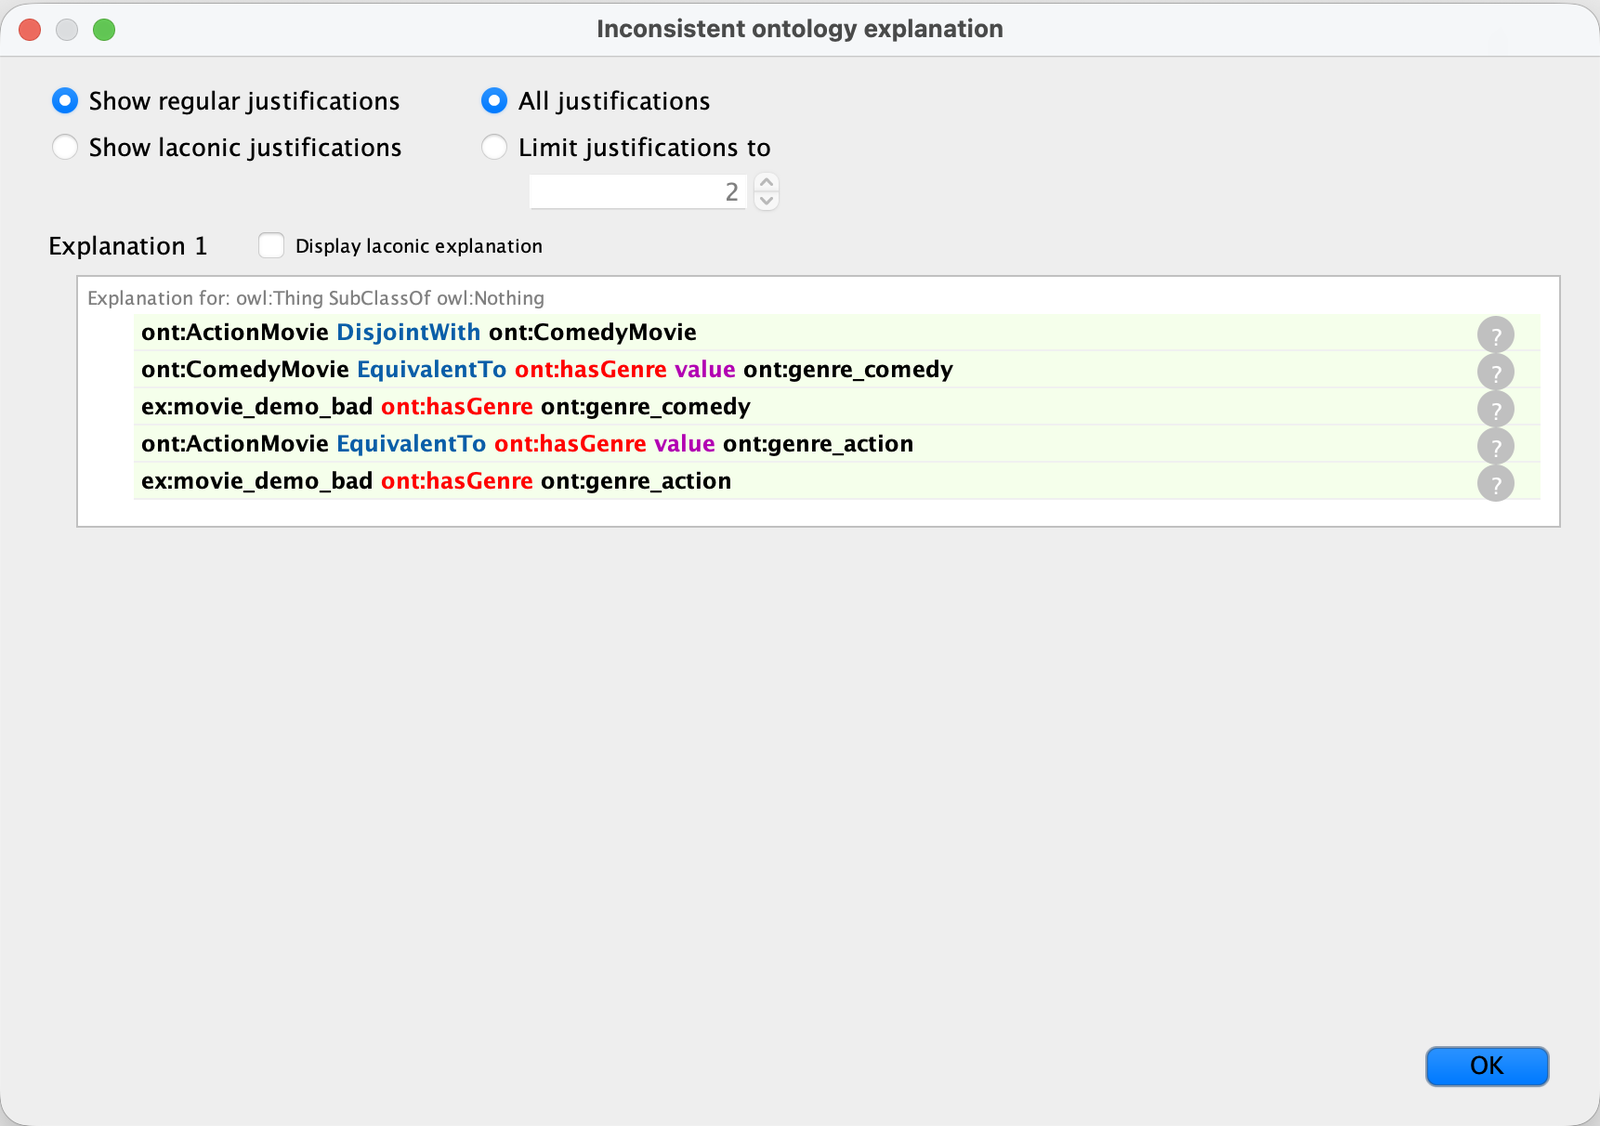
\includegraphics[width=0.78\textwidth]{fig/fig3-explain.png}
\caption{Protégé's explanation of the inconsistency caused by a film with two disjoint genres.}\label{fig:explain}
\end{figure}

% ---------------------------------------------------------------- 8
\section{Dataset Metadata}\label{sec:metadata}

Following the W3C recommendations for publishing data on the Web, the dataset describes itself in \code{dataset\_metadata.ttl}, generated by a script from the actual files: DCAT~\cite{dcat} for the catalogue, the dataset and one distribution per Turtle file; VoID~\cite{void} for statistics and two linksets (920 links to Wikidata, 912 to DBpedia); and PROV-O~\cite{provo} for provenance, recording that the dataset was derived from the two Kaggle files by one pipeline activity that used Wikidata, DBpedia and our scripts. Licences are stated per part: MIT for the code, CC BY-NC 4.0 for our RDF, the TMDb terms for the upstream facts, CC0 for Wikidata links and CC BY-SA for DBpedia links.

% ---------------------------------------------------------------- 9
\section{Discussion and Limitations}

Two lessons stand out. First, matching on shared identifiers is far more reliable than matching on names: the identifier-based method linked 99.6\% of films to both hubs, whereas title-based matching found nothing. Second, \code{owl:sameAs} statements imported from a large source must be verified: redirect resources silently assert identity between different entities, and a small manual sample was enough to expose the problem.

The project has the following limitations:
\begin{itemize}
  \item \code{Director} and \code{Actor} are modelled as subclasses although they are roles.
  \item Only the primary genre of each film is kept, to keep the disjoint genre classes consistent.
  \item The URIs use \code{example.org} and cannot be dereferenced on the Web.
  \item \code{characterName} is a literal: TMDB gives only a name, so different characters with the same name cannot be distinguished.
  \item The dataset is a snapshot of 250 films, and two resources remain unlinked because their identifiers are ambiguous.
\end{itemize}

\section{Conclusion and Future Work}

We built a five-star Linked Open Data set of 250 films: an ontology that reuses standard vocabularies and supports reasoning, RDF with stable URIs, 1,832 identifier-based links to Wikidata and DBpedia with a measured precision of 96.7--100\%, and 21 SPARQL queries, ten of them federated. Future work includes modelling roles with a \code{hasRole} property, keeping all genres with non-disjoint genre classes, publishing the data with dereferenceable URIs behind a SPARQL endpoint such as Apache Jena Fuseki, and extending the dataset with more films and awards.

% ---------------------------------------------------------------- team
\section*{Team Contributions}
\addcontentsline{toc}{section}{Team Contributions}
\begin{table}[H]
\centering\small
\begin{tabularx}{\textwidth}{@{}l>{\raggedright\arraybackslash}X@{}}
\toprule
Member & Contributions \\
\midrule
Đỗ Tuấn Minh (leader) & Ontology design, defined classes and SWRL rule, reasoning checks, awards from Wikidata, terminal SPARQL interface, demo \\
Nguyễn Tiến Đức & Data collection and cleaning, CSV-to-RDF conversion, Wikidata and DBpedia linking and its redirect correction, link evaluation, statistics, slides \\
Hoàng Huy Chiến & Dataset metadata, federated queries, the CastRole model and its queries, report, demo video \\
\bottomrule
\end{tabularx}
\end{table}

% ---------------------------------------------------------------- references
\begin{thebibliography}{99}\small
\bibitem{fivestar} T.~Berners-Lee. \emph{Linked Data --- Design Issues}, W3C, 2006 (five-star scheme added 2010). \url{https://www.w3.org/DesignIssues/LinkedData.html}; see also \url{https://5stardata.info/}.
\bibitem{bizer2009linked} C.~Bizer, T.~Heath, T.~Berners-Lee. Linked Data --- The Story So Far. \emph{International Journal on Semantic Web and Information Systems}, 5(3):1--22, 2009.
\bibitem{dbpedia} J.~Lehmann et al. DBpedia --- A large-scale, multilingual knowledge base extracted from Wikipedia. \emph{Semantic Web}, 6(2):167--195, 2015.
\bibitem{wikidata} D.~Vrandečić, M.~Krötzsch. Wikidata: a free collaborative knowledgebase. \emph{Communications of the ACM}, 57(10):78--85, 2014.
\bibitem{methontology} M.~Fernández-López, A.~Gómez-Pérez, N.~Juristo. METHONTOLOGY: From ontological art towards ontological engineering. \emph{AAAI Spring Symposium on Ontological Engineering}, 1997.
\bibitem{gruninger1995} M.~Grüninger, M.\,S.~Fox. Methodology for the design and evaluation of ontologies. \emph{IJCAI Workshop on Basic Ontological Issues in Knowledge Sharing}, 1995.
\bibitem{ontoclean} N.~Guarino, C.~Welty. Evaluating ontological decisions with OntoClean. \emph{Communications of the ACM}, 45(2):61--65, 2002.
\bibitem{swrl} I.~Horrocks et al. SWRL: A Semantic Web Rule Language Combining OWL and RuleML. W3C Member Submission, 2004.
\bibitem{naryrel} N.~Noy, A.~Rector (eds.). Defining N-ary Relations on the Semantic Web. W3C Working Group Note, 2006.
\bibitem{halpin2010sameas} H.~Halpin, P.\,J.~Hayes, J.\,P.~McCusker, D.\,L.~McGuinness, H.\,S.~Thompson. When owl:sameAs isn't the same: An analysis of identity in Linked Data. \emph{ISWC}, 2010.
\bibitem{hermit} B.~Glimm, I.~Horrocks, B.~Motik, G.~Stoilos, Z.~Wang. HermiT: An OWL 2 Reasoner. \emph{Journal of Automated Reasoning}, 53(3):245--269, 2014.
\bibitem{protege} M.\,A.~Musen. The Protégé project: a look back and a look forward. \emph{AI Matters}, 1(4):4--12, 2015.
\bibitem{dcat} W3C. Data Catalog Vocabulary (DCAT) --- Version 3. W3C Recommendation, 2024.
\bibitem{void} K.~Alexander, R.~Cyganiak, M.~Hausenblas, J.~Zhao. Describing Linked Datasets with the VoID Vocabulary. W3C Interest Group Note, 2011.
\bibitem{provo} T.~Lebo, S.~Sahoo, D.~McGuinness (eds.). PROV-O: The PROV Ontology. W3C Recommendation, 2013.
\bibitem{tmdb5000} The Movie Database (TMDb). TMDB 5000 Movie Dataset, Kaggle. \url{https://www.kaggle.com/datasets/tmdb/tmdb-movie-metadata}.
\end{thebibliography}

\end{document}
